% ===========================================================================
%  09 -- 附录
% ===========================================================================
\chapter{附录}\label{ch:appendix}

本附录为方法论、实现和评估章节提供支持材料。它保留了原始配置、数据集、回放、图表和试点编码材料，而不扩展主章节中所述的声明边界。

% ===========================================================================
\section{完整 LoRA 超参数配置}\label{sec:appendix-hyperparams}

表~\ref{tab:lora-hyperparams-full} 列出了在匹配的 Run-003 + Run-005$\times$2 配方下三种骨干模型的完整超参数配置。数值来自可用的训练报告和基准测试工件。

\begin{table}[htbp]
  \centering
  \caption{三种骨干的完整 LoRA 微调超参数。}
  \label{tab:lora-hyperparams-full}
  \small
  \begin{tabular}{@{}llll@{}}
  \toprule
  \textbf{参数} & \textbf{Qwen3.5-9B} & \textbf{Qwen3.6-27B} & \textbf{Gemma-4-31B} \\
  \midrule
  \texttt{max\_seq\_length} & 4096 & 4096 & 4096 \\
  \texttt{num\_train\_epochs} & 4.0 & 4.0 & 4.0 \\
  \texttt{learning\_rate} & $2{\times}10^{-4}$ & $2{\times}10^{-4}$ & $2{\times}10^{-4}$ \\
  \texttt{per\_device\_train\_batch\_size} & 1 & 1 & 1 \\
  \texttt{gradient\_accumulation\_steps} & 4 & 4 & 4 \\
  \texttt{lora\_r} & 16 & 16 & 16 \\
  \texttt{lora\_alpha} & 16 & 16 & 16 \\
  \texttt{lora\_dropout} & 0.0 & 0.0 & 0.0 \\
  \texttt{seed} & 3407 & 3407 & 3407 \\
  \texttt{load\_in\_4bit} & True & True & True \\
  \texttt{warmup\_ratio} & 0.1 & 0.1 & 0.1 \\
  \texttt{weight\_decay} & 0.01 & 0.01 & 0.01 \\
  \texttt{train\_rows} & 928 & 928 & 928 \\
  \texttt{eval\_rows} & 0 & 0 & 0 \\
  \midrule
  \textbf{骨干特定} & & & \\
  \midrule
  Vision LoRA & 启用 & 启用 & 禁用 \\
  LoRA 目标模块 & vision+lang & vision+lang & all-linear \\
  对话模板 & Qwen 默认 & Qwen 默认 & gemma-4 \\
  GPU 内存利用率 & 0.6 & 0.6 & 0.95 \\
  \midrule
  \textbf{训练结果} & & & \\
  \midrule
  训练运行时间 (s) & 6419 & 12619 & 8050 \\
  训练损失 (最终) & 0.2156 & 0.1068 & 0.0474 \\
  \bottomrule
  \end{tabular}
\end{table}

注意：由于分词器行为、对话模板结构、目标序列分布和模型参数化的差异，训练损失值在不同骨干之间不可直接比较。

% ===========================================================================
\section{8 事实 V1 基线基准测试}\label{sec:appendix-8fact}

最早的完整基准测试使用在 Run-001（180 个任务）上训练并在 Run-002 留存集（50 个样本）上评估的 8 事实 LoRA 适配器。该线早于 13 事实本体，在此作为历史参考收录。

\begin{table}[htbp]
\centering
\caption{8 事实 v1 基准测试：Qwen3.5-9B 基座 vs.\ LoRA-v1 在 Run-002 留存集上的对比（50 样本，EN）。}\label{tab:appendix-qwen-8fact}
\begin{tabular}{l c c c}
\toprule
\textbf{指标} & \textbf{基座} & \textbf{LoRA-v1} & \textbf{$\Delta$} \\
\midrule
JSON 有效率       & 1.0    & 1.0    & --- \\
Schema 有效率     & 1.0    & 1.0    & --- \\
事实准确率         & 0.7600 & 0.9150 & +0.1550 \\
宏平均 $F_1$      & 0.4241 & 0.5847 & +0.1605 \\
Seen $F_1$        & 0.4714 & 0.8380 & +0.3666 \\
样本完全匹配       & 0.06   & 0.36   & +0.30 \\
关键假阳性        & 13  & 15     & +2 \\
\bottomrule
\end{tabular}
\end{table}

% 证据：benchmarks/qwen35_vlm_finetune/base_vs_lora_holdout_run002_v1/

LoRA 适配器大幅提升了事实级指标，但将关键假阳性从 13 增加到 15。这一历史结果说明了 8 事实 v1 本体的结构性弱点：诸如 \texttt{ins\_go} 等复合目标无法从单帧中视觉验证，并在完成型事实上产生了系统性的假阳性错误。

% ===========================================================================
\section{数据集事实分布}\label{sec:appendix-datasets}

表~\ref{tab:fact-distributions} 报告了两个主要训练来源（Run-003、Run-005）和两个 13 事实留存集（Run-002 newfacts、Run-004 random）中每个事实的 \texttt{seen} 计数。计数来自对应的 \texttt{stats.json} 文件。表格使用简短显示标签；权威的事实标识符定义在程序包使用的视觉事实本体文件中。

\begin{table}[htbp]
\centering
\caption{训练集与留存数据集中每个事实的 \texttt{seen} 计数（13 事实 v2 本体）。}
\label{tab:fact-distributions}
\small
\begin{tabularx}{\textwidth}{@{}>{\raggedright\arraybackslash}Xrrrr@{}}
\toprule
\textbf{事实标签} & \textbf{Run-003} & \textbf{Run-005} & \textbf{Run-002} & \textbf{Run-004} \\
\midrule
TAC 页面可见            & 46  & 24  & 23 & 3  \\
SUPT 页面可见           & 20  & 34  & 5  & 3  \\
FCS 页面可见            & 30  & 40  & 13 & 94 \\
FCS X 标记可见         & 16  & 18  & 1  & 5  \\
BIT 根页面可见       & 18  & 43  & 9  & 16 \\
FCS-MC 页面可见         & 55  & 56  & 9  & 84 \\
FCS-MC 中间结果  & 18  & 15  & 1  & 7  \\
FCS-MC 测试中状态       & 18  & 19  & 6  & 17 \\
FCS-MC 最终 GO 结果      & 18  & 22  & 2  & 60 \\
HSI 页面可见            & 106 & 109 & 49 & 100 \\
HSI 地图图层可见       & 79  & 37  & 27 & 50 \\
INS GRND 对准文本     & 58  & 72  & 42 & 69 \\
INS OK 文本                 & 12  & 14  & 4  & 0  \\
\bottomrule
\end{tabularx}
\end{table}

% 证据：datasets/vision_sft_run003/stats.json,
%           datasets/vision_sft_run005_composition_rebalance/stats.json,
%           datasets/vision_sft_holdout_run002_newfacts/stats.json,
%           datasets/vision_sft_holdout_run004_random/stats.json

Run-005 在与 Run-003 组合时为多个稀疏目标增加了覆盖：SUPT 页面观察从 20 增加到 54，FCS-MC 页面观察从 55 增加到 111，INS GRND 对准文本观察从 58 增加到 130。本表记录了数据来源；第~\ref{ch:evaluation}~章评估了所得训练配方是否改善了模型在留存集上的行为。

% ===========================================================================
\section{CLI 命令参考}\label{sec:appendix-cli}

\texttt{simtutor} 包提供以下 CLI 命令：

\begin{description}
\item[\texttt{run}.] 使用模拟环境适配器以预录制的场景文件执行仿真并写入事件日志。
\item[\texttt{replay}.] 对照程序包验证现有事件日志，检查步骤顺序和状态机一致性。
\item[\texttt{score}.] 使用评分引擎对事件日志进行评分，生成遗漏计数、状态违反计数和总错误分数。
\item[\texttt{record-vlm}.] 在一组视觉观察上运行 VLM 事实提取，并记录预测结果用于基准测试。
\item[\texttt{replay-bios}.] 将原始 DCS-BIOS 捕获数据通过遥测流水线回放，并可选择性地调用帮助生成循环。
\item[\texttt{validate}.] 对照 Schema 注册表中的命名 Schema 验证 JSONL 文件。
\end{description}

所有命令均接受模型配置覆盖参数（\texttt{--model-provider}、\texttt{--model-name}、\texttt{--model-base-url}、\texttt{--model-timeout-s}）和语言切换参数（\texttt{--lang}）。

% ===========================================================================
\section{模型提供方配置}\label{sec:appendix-model-config}

模型访问通过环境变量配置并在运行时验证：

\begin{description}
\item[提供方。] \texttt{SIMTUTOR\_MODEL\_PROVIDER} 选择 \texttt{openai\_compat}、\texttt{ollama} 或 \texttt{stub}。
\item[基础 URL。] \texttt{SIMTUTOR\_MODEL\_BASE\_URL} 设置提供方端点。
\item[模型。] \texttt{SIMTUTOR\_MODEL\_NAME} 选择模型名称。
\item[超时。] \texttt{SIMTUTOR\_MODEL\_TIMEOUT\_S} 设置请求超时时间。
\item[凭证。] \texttt{SIMTUTOR\_MODEL\_API\_KEY} 是 \texttt{openai\_compat} 提供方所必需的。API 密钥在日志输出中被遮蔽。
\item[图像。] \texttt{SIMTUTOR\_MODEL\_ENABLE\_MULTIMODAL} 切换请求中的 base64 图像编码。
\item[语言。] \texttt{SIMTUTOR\_LANG} 选择 \texttt{zh} 或 \texttt{en}。
\end{description}

% ===========================================================================
\section{回放评估套件}\label{sec:appendix-replay}

表~\ref{tab:replay-cases} 列出了 \texttt{fa18c\_startup\_v04} 套件中的五个回放评估案例。此处显示标签已缩短；套件文件保留了确切的 \texttt{case\_id} 字符串。

\begin{table}[htbp]
\centering
\caption{回放评估案例。}
\label{tab:replay-cases}
\small
\begin{tabularx}{\textwidth}{@{}>{\raggedright\arraybackslash}Xccl@{}}
\toprule
\textbf{案例} & \textbf{步骤} & \textbf{视觉} & \textbf{目标} \\
\midrule
空操作捕获 & S01 & 否 & 电池开关 \\
电池接通 & S02 & 否 & 火警测试开关 \\
电池接通，发动机发电机关闭 & S01 & 否 & 左发电机开关 \\
FCS 重置 / FCS BIT & S18 & 是 & FCS BIT 开关 \\
INS 模式 & S12 & 是 & INS 模式旋钮 \\
\bottomrule
\end{tabularx}
\end{table}

% 证据：replay_eval/fa18c_startup_v04/suite.yaml

标记为视觉可用的案例在对应的 DCS Saved Games 捕获中包含每帧侧车文件（\texttt{frames.jsonl}）。这些文件允许依赖视觉的回放案例在无实时 DCS 实例的情况下运行。

% ===========================================================================
\section{补充架构与导出图表}\label{sec:appendix-figures}

主章节使用简化的图表来支持研究论证。图~\ref{fig:harness-validation}、\ref{fig:deployment-topology} 和 \ref{fig:experiment-export} 保留了额外的工程细节，以确保可复现性和操作上下文。

\begin{figure}[htbp]
  \centering
  
\includegraphics[width=\textwidth]{figures/fig_harness_validation.pdf}
  \caption{安全约束与证据验证。候选教学系统动作在被接受为叠加层动作计划之前，需经过 Schema 约束、UI 白名单、证据一致性和程序状态的检查；不安全或证据不够充分的动作将被修复、拒绝或降级为纯文本指导。}
  \label{fig:harness-validation}
\end{figure}

\begin{figure}[htbp]
  \centering
  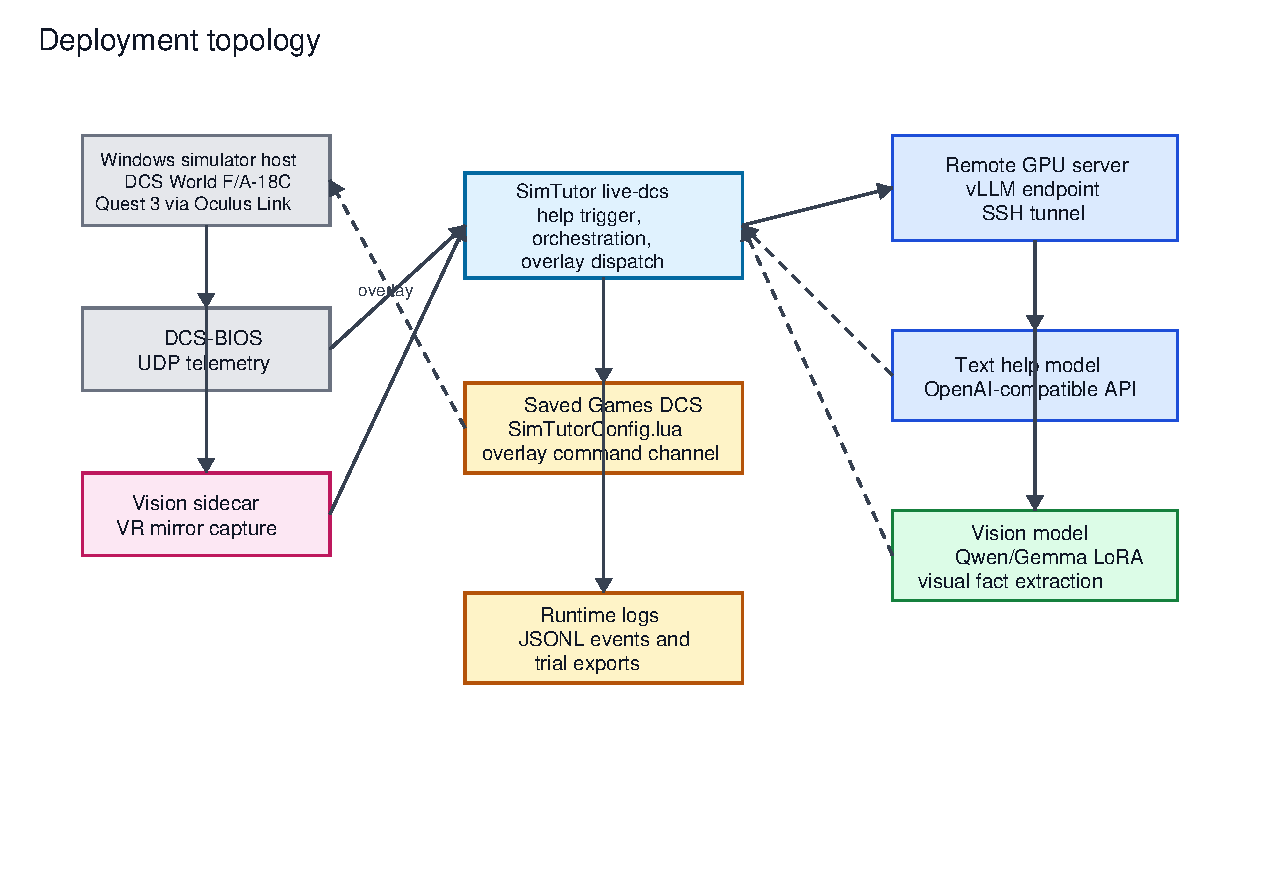
\includegraphics[width=\textwidth]{figures/fig_deployment_topology.pdf}
  \caption{原型所使用的部署拓扑。仿真器、Quest 3 叠加层通道、本地运行时、回放工具和远程模型提供方被区分开来，使得实时试验和离线分析可以使用相同的证据和日志记录契约。}
  \label{fig:deployment-topology}
\end{figure}

\begin{figure}[htbp]
  \centering
  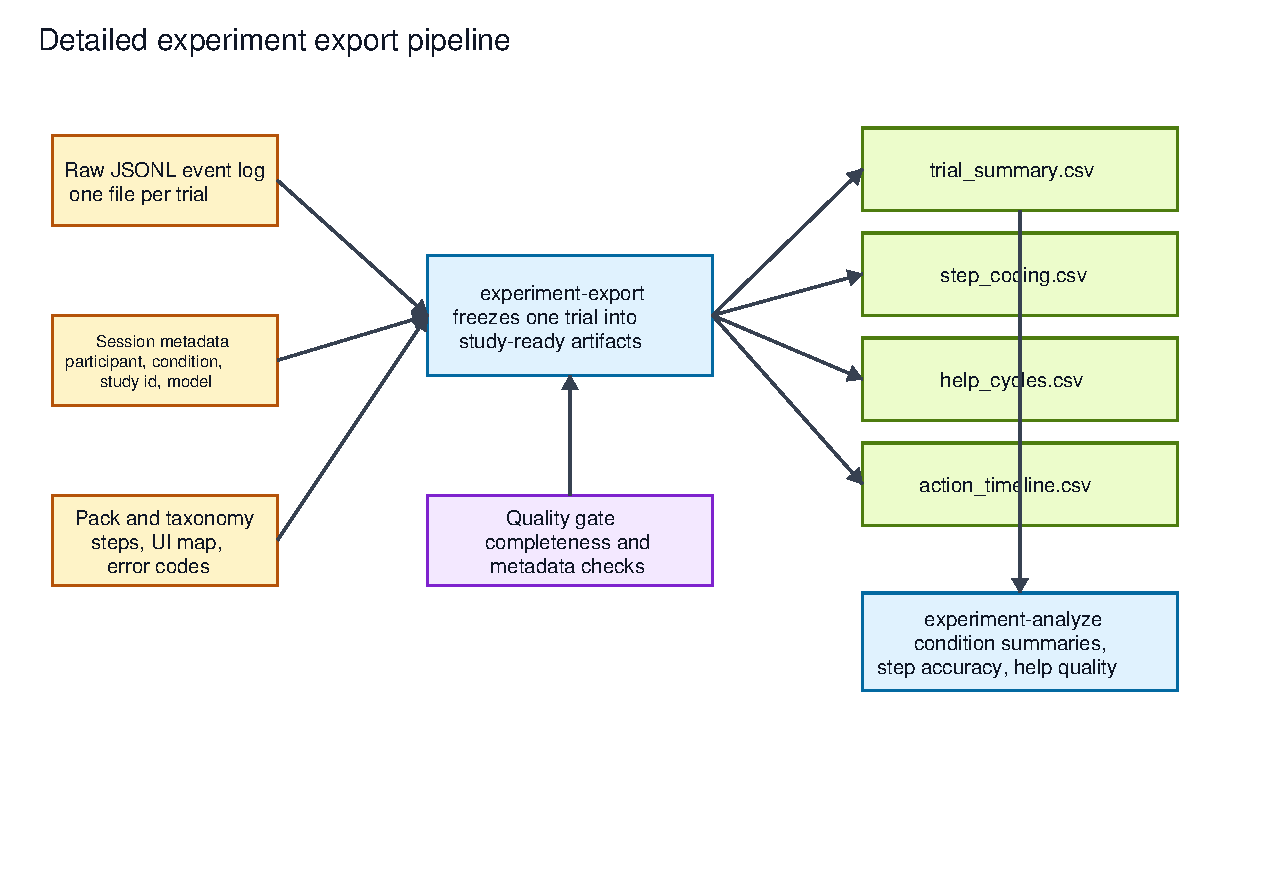
\includegraphics[width=\textwidth]{figures/fig_experiment_export.pdf}
  \caption[详细的实验导出流水线]{详细的实验导出流水线。运行时事件日志和试验元数据被转换为参与者级摘要、步骤编码、帮助循环记录、质量门控和研究级分析表。}
  \label{fig:experiment-export}
\end{figure}

% ===========================================================================
\section{VR 试点研究 --- 补充数据}\label{sec:appendix-pilot}

表~\ref{tab:pilot-participants} 列出了参与者经验概况。

\begin{table}[htbp]
\centering
\caption{试点参与者经验概况（自报告）。}\label{tab:pilot-participants}
\small
\begin{tabularx}{\textwidth}{@{}ll>{\raggedright\arraybackslash}Xl@{}}
\toprule
\textbf{P} & \textbf{条件} & \textbf{自报告经验} & \textbf{分组} \\
\midrule
P01 & 无教学系统 & DCS 频繁；飞行模拟频繁；VR 频繁；Quest 3 频繁 & 中级 \\
P02 & 无教学系统 & DCS 中级；飞行模拟中级；VR 频繁；Quest 3 频繁 & 未记录 \\
P03 & 无教学系统 & DCS 新手；飞行模拟新手；VR 中级；Quest 3 频繁 & 入门 \\
P04 & 有教学系统 & DCS 中级；飞行模拟中级；VR 频繁；Quest 3 频繁 & 中级 \\
P05 & 有教学系统 & DCS 中级；飞行模拟中级；VR 频繁；Quest 3 频繁 & 未记录 \\
P06 & 无教学系统 & DCS 新手；飞行模拟新手；VR 中级；Quest 3 频繁 & 入门 \\
P07 & 无教学系统 & DCS 新手；飞行模拟新手；VR 中级；Quest 3 频繁 & 入门 \\
P08 & 有教学系统 & DCS 新手；飞行模拟新手；VR 频繁；Quest 3 频繁 & 未记录 \\
P09 & 有教学系统 & DCS 新手；飞行模拟新手；VR 中级；Quest 3 中级 & 入门 \\
\bottomrule
\end{tabularx}

未记录 = 未记录。
\end{table}

表~\ref{tab:pilot-uncompleted} 列出了每位无教学系统辅助参与者未完成的具体步骤。

\begin{table}[htbp]
\centering
\caption{无教学系统辅助条件下未完成的步骤（手动编码）。}\label{tab:pilot-uncompleted}
\small
\begin{tabularx}{\textwidth}{@{}l>{\raggedright\arraybackslash}X@{}}
\toprule
\textbf{P} & \textbf{未完成的步骤} \\
\midrule
P01 & S09、S12、S18、S19、S20、S22、S24、S27、S29、S31 \\
P02 & S02、S14、S18、S19、S27、S30 \\
P03 & S07、S09、S16、S18、S19、S26、S27、S29、S32 \\
P06 & S07、S18、S19、S27 \\
P07 & S02、S09、S12、S13、S16、S17、S18、S19、S22、S26、S27、S28、S29、S32 \\
\bottomrule
\end{tabularx}

S18（右 DDI 上的 FCS-MC BIT 页面）和 S19（FCS BIT 最终 GO 结果）被所有五名无教学系统辅助参与者遗漏，且属于视觉优先的显示检查。S27（襟翼开关置于 AUTO）同样被所有五名参与者遗漏，但程序包将其归类为 BIOS 优先，使用变量和门控证据而非 VLM 约束的视觉证据。因此，该模式是描述性的：它显示了参与者在哪些地方遇到困难，而非某一种证据源能够解释遗漏。
\end{table}

表~\ref{tab:pilot-errors-auto} 报告了自动编码的错误计数（手动审查前）与手动错误计数的对比，显示了在试点解读之前自动导出结果有多少需要被纠正。

\begin{table}[htbp]
\centering
\caption{每位参与者的自动编码 vs.\ 手动错误计数。}\label{tab:pilot-errors-auto}
\small
\begin{tabular}{@{}llrrrrr@{}}
\toprule
\textbf{P} & \textbf{条件} & \textbf{自动遗漏} & \textbf{自动执行} & \textbf{手动遗漏} & \textbf{手动执行} & \textbf{手动总计} \\
\midrule
P01 & 无教学系统 & 4  & 3  & 8  & 0 & 10 \\
P02 & 无教学系统 & 0  & 3  & 0  & 0 & 1  \\
P03 & 无教学系统 & 0  & 4  & 7  & 0 & 11 \\
P06 & 无教学系统 & 0  & 3  & 2  & 0 & 4  \\
P07 & 无教学系统 & 1  & 9  & 11 & 0 & 11 \\
P04 & 有教学系统 & 0  & 4  & 0  & 3 & 7  \\
P05 & 有教学系统 & 0  & 3  & 0  & 3 & 6  \\
P08 & 有教学系统 & 0  & 3  & 0  & 0 & 0  \\
P09 & 有教学系统 & 0  & 3  & 0  & 3 & 5  \\
\bottomrule
\end{tabular}

自动编码错误来自自动化流水线（\texttt{step\_coding.csv} 中的 Auto\_Error\_* 列）。手动错误来自经人工审查的列（Error\_*）。P08 的自动错误经手动审查后全部被覆盖为零（参见第~\ref{sec:eval-pilot}~节中的数据质量说明）。
\end{table}
